% =========================================================
% fpga-results.tex
% =========================================================
% The results obtained with the FPGA implementations of
% Kyber

\section*{Evaluation}

To quantitatively understand our design and the impact of
our design choices, we pushed both the implementation of
the entire design, as well as the more-optimized NTT kernel
(including the NTT and INVNTT operations),
through the FPGA flow and implemented on the class Zynq FPGA.
This gave us both results after synthesis, as well as a
bitstream to use on an FPGA to gain experimental results,
allowing us to better gain takeaways about the efficacy of
our design.

% ---------------------------------------------------------
% Synthesis
% ---------------------------------------------------------
% Results obtained solely from synthesis

\subsection*{Synthesis}

The first step to gain quantitative results is to use
Vivado's HLS flow to push both of our implementations
through the FPGA flow. This can tell us how many hardware
resources the designs would need, as well as a prediction
of how long each design will take. This is shown in Figures
\ref{fig:results-synth-util} and \ref{fig:results-synth-lat},
respectively.

\begin{figure}[H]
  \centering
  \begin{subfigure}{.45\textwidth}
    \centering
    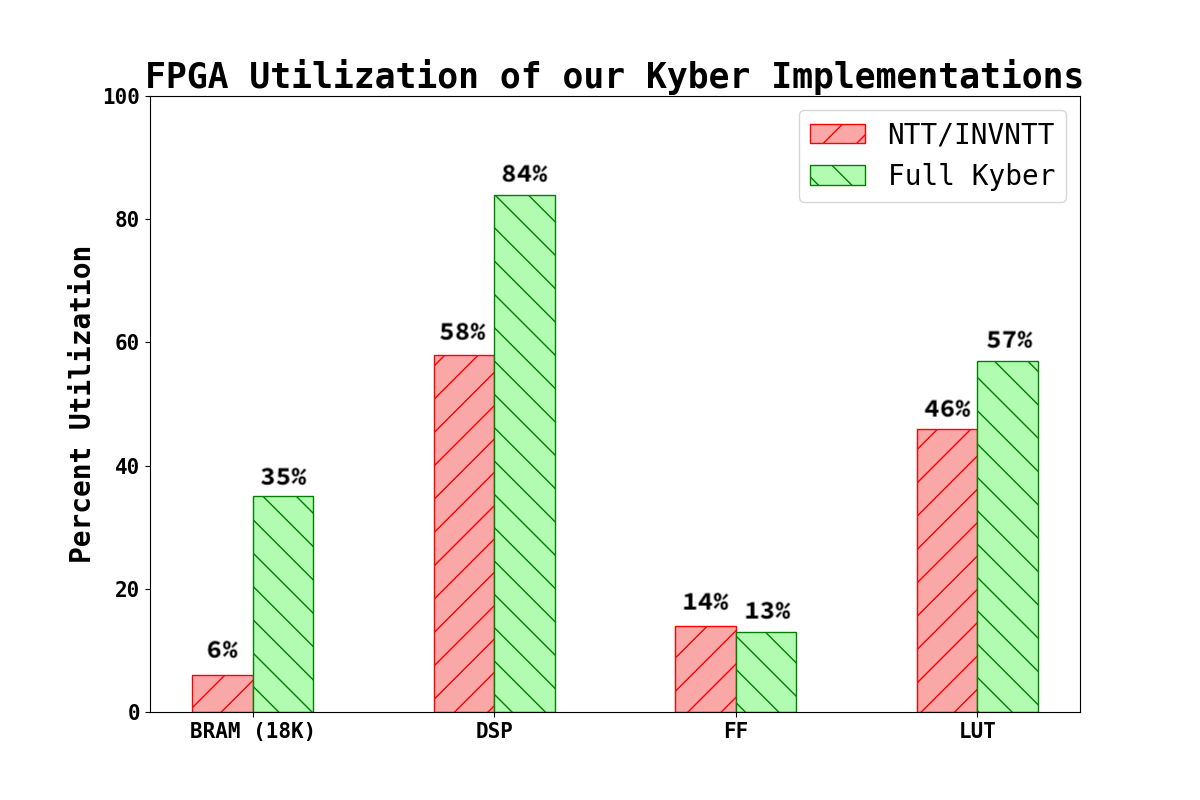
\includegraphics[width=\linewidth]{imgs/results-synth-util.png}
    \caption{The hardware utilization of the different FPGA implementations}
    \label{fig:results-synth-util}
  \end{subfigure}\hspace{0.05\textwidth}%
  \begin{subfigure}{.45\textwidth}
    \centering
    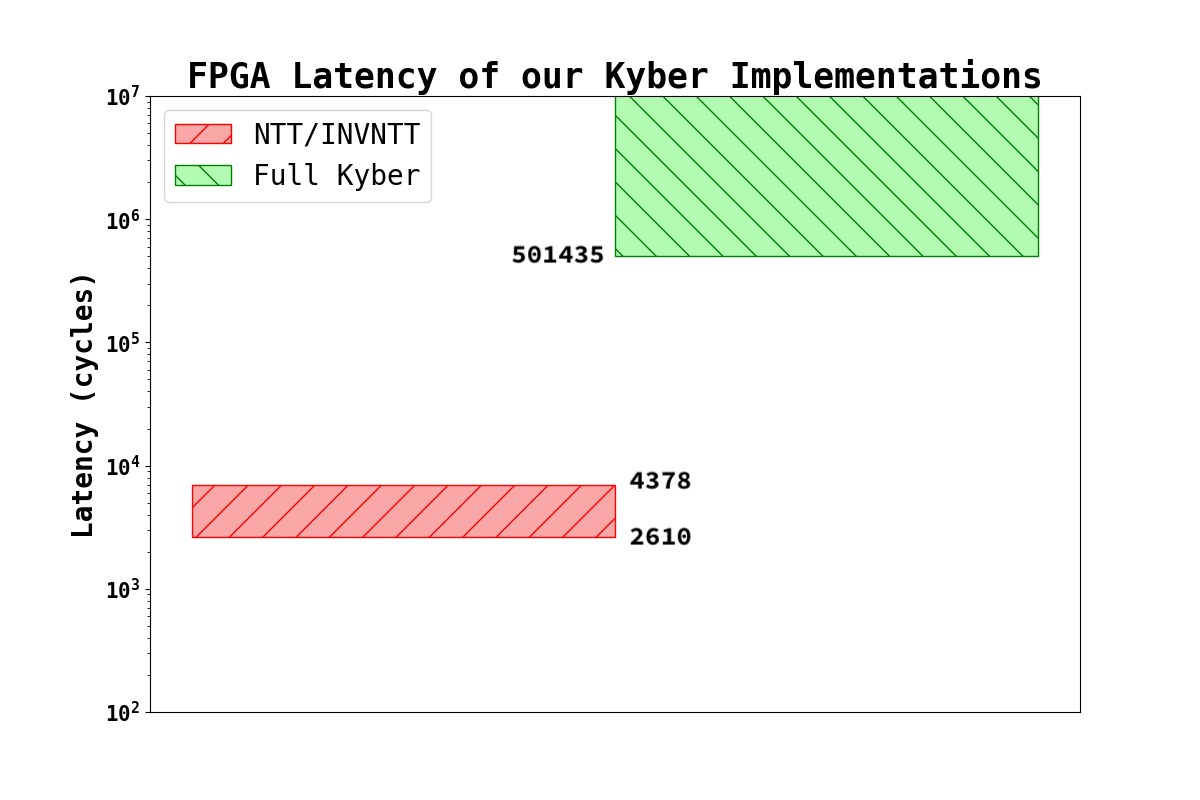
\includegraphics[width=\linewidth]{imgs/results-synth-lat.png}
    \caption{The expected latency of the different FPGA implementations}
    \label{fig:results-synth-lat}
  \end{subfigure}
  \caption{The synthesis results for our FPGA implementations}
\end{figure}

For the utilization in Figure \ref{fig:results-synth-util},
we can see that putting the entire design on FPGA hardware
results in more hardware resources overall, as expected.
One interesting note is the overall amount of DSP usage; for
both designs, a significant number are used, much more than
other labs have seen. This is due to the need for multipliers
in Montgomery conversion. Having a value in Montgomery form
can change performing a modulus over one value (as needed
for modular ring operations) to another;
by choosing to perform a modulus over a power of two, such
moduli can be implemented in hardware quickly. However,
converting in and out of this representation involves a
multiplication step. This particular operation was one of
the key reasons why the NTT kernel couldn't be as
optimized. The NTT kernel had an outer loop that required
a Montgomery conversion for each iteration, where the
number of iterations varied each time it was used. Although
we could unroll most uses of this loop, the largest version
of this loop could not be unrolled, due to the limited
number of DSP blocks available.

While the entire design used more resources in general, we
also discovered that the optimized NTT kernel surprisingly
used \textit{more} flip-flops (\code{FF}) compared to the
overall design. This seems somewhat surprising, considering
that the NTT kernels are included (multiple times) in the
entire algorithm, but makes sense once you consider the
extra optimizations applied to the NTT algorithms in
isolation. Specifically, with just the NTT algorithms, we
can exploit loop pipelining and unrolling to achieve much
higher performance by doing operations in parallel; however,
this comes at the cost of extra flip-flops to store
intermediate results in the different pipeline stages, as
well as replicated across all loop iterations. This contrasts
with the entire design in hardware; due to the lack of
available resources, we are able to optimized the design
much less, reducing the number of flip-flops needed in
this case from the lack of aggressive pipelining/unrolling.

In addition to the hardware utilization of each design, we
also compare about the predicted latency of each design;
how many cycles each design should take. This is shown as a
range for both designs in Figure \ref{fig:results-synth-lat}. For the NTT
algorithms, the latency is uncertain, as it depends on which
operation we're performing. Performing an NTT operation takes
\textbf{2610 cycles}, whereas performing an INVNTT operation takes
\textbf{4378 cycles} due to an extra multiplication reduction step needed at
the end. However, for the entire design, the lowest latency
was \textbf{501453 cycles} (on the order as expected), but the tools
could not compute an upper latency bound. When we fixed the
offending loops to have constant bounds, the maximum possible
latency was astronomical (on the order of ~1000 seconds). This
is because the algorithm currently uses rejection sampling to
achieve a random number in the modular ring for Kyber. In
practice, many rejections are likely not needed (or algorithmic
changes could be made to use a modulus instead of random
sampling, albeit affecting the distribution), so our design
can be best approximated by the lower bound.

% ---------------------------------------------------------
% Experimental
% ---------------------------------------------------------
% Results obtained from running the implementation on the
% FPGA

\subsection*{Experimental}

In addition to theoretical results, we additionally used
Vivado's HLS tools to generate bitstreams for both
implementations, such that they could be used on the FPGA.
This allowed us to write host-side code to run on the ARM
core and interact with our designs to measure their actual
execution time, the results of which are shown in Figure
\ref{fig:results-exp-time}. Measurements were done by running
the desired algorithm 20 times by feeding 20 inputs, then
reading the resulting 20 outputs, in order to amortize the
communication latency.

\begin{figure}[H]
  \centering
  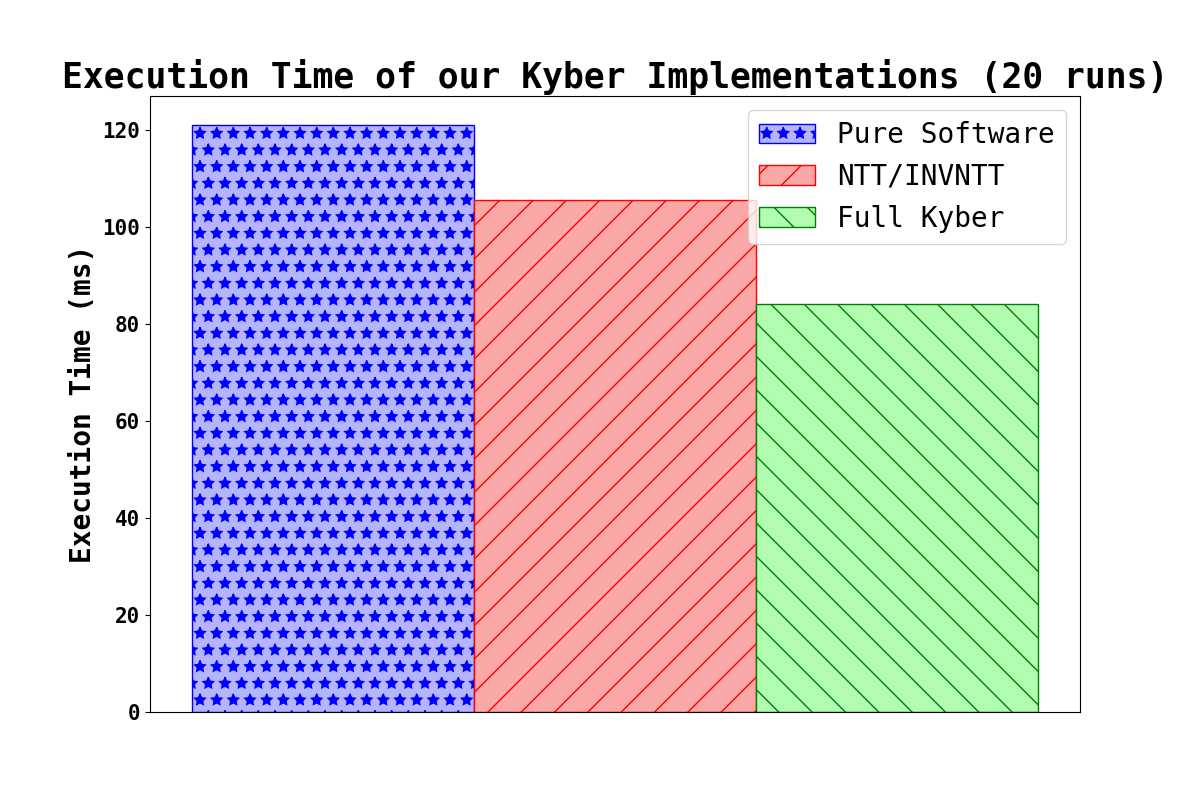
\includegraphics[width=0.5\linewidth]{imgs/results-exp-time.png}
  \caption{
    The measured execution time of the different Kyber
    implementations on the FPGA
  }
  \label{fig:results-exp-time}
\end{figure}

From the figure, we can see that the NTT algorithms in hardware
(taking \textbf{105.463 ms}) resulted in some speedup over a pure
software implementation (\textbf{120.859 ms}), but were overall
limited in their speedup from the fact that the majority of the
Kyber algorithm was still in software. Even though we significantly
optimized the NTT/INVNTT portions of the algorithm, they only
composed an overall (\textbf{28.354 ms}) of the algorithm, with
the other (\textbf{77.108 ms}) representing the remaining (unoptimized)
software algorithm.

Having the entire algorithm in hardware (\textbf{84.050 ms}) resulted
in more speedup over software than just the NTT kernels, but ultimately
not as much as we hoped. This is due to two main factors:

\begin{itemize}
  \item The ARM core is running at a faster frequency than the FPGA
        fabric. Therefore, software algorithms, even though running on
        general-purpose hardware, may be more competitive due to their
        higher frequency
  \item Kyber is composed of many different kernels and parts of the
        algorithm, as shown in the flame graph above. Each of these
        different operations requires different hardware to implement,
        resulting in low levels of hardware re-use. Because of this,
        many resources are used to simply implement the entire algorithm,
        leaving fewer available to parallelize the operations for higher
        performance, as was achieved in lab. We were ultimately unable to
        optimize large portions of the design for this reason.
\end{itemize}

